\chapter{The Hall Effects}

\label{chapter2}

\section{Introduction - Ordinary Hall effect}

These effects originally deal with the application of an external magnetic field on a current carrying material and subsequently observing the effect either on the conductor or the electric current itself.

In 1879, Edwin Hall was exploring this interaction and tried to determine the effect of the magnetic field on a current carrying wire, with a suspicion that it either affected the whole length of the wire or only the moving electrons.

He later devised a rather simple experiment based on the argument that ``if the current of electricity in a fixed conductor is itself attracted by a magnet, the current should be drawn to one side of the wire, and therefore the resistance experienced should be increased." \autocite[1]{S.1880}

Hall couldn't detect this extra resistance (which we now know as magnetoresistance) but concluded that a transverse force in the opposite direction must exist and which appears as a transverse voltage across the width of the conducting material. This is the Hall effect and the transverse voltage is the Hall voltage.

The experiment by Hall is shown in the figure below.

\begin{figure}
    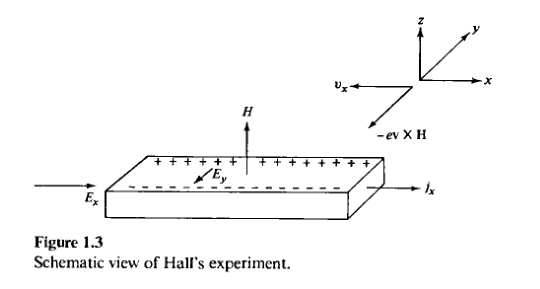
\includegraphics[width=\columnwidth]{hall-effect-ashcroft.png}
    \caption{Schematic diagram of the Hall effect}
\end{figure}

\subsection{Mathematical analysis}

In the given figure, an electric current is passed along the $ x $ direction with corresponding current density as $ j_x $. The cause of this current is an external electric field along the same direction $ E_x $.

An external magnetic field $ H $ along the $ z $ direction is applied and the Hall effect is observed.


